\documentclass[12pt, a4paper]{article}

% -- Packages --
\usepackage[utf8]{inputenc}
\usepackage[T1]{fontenc}
\usepackage{amsmath, amssymb, amsthm}
\usepackage{graphicx}
\usepackage{booktabs}
\usepackage{hyperref}
\usepackage[margin=1in]{geometry}
\usepackage{caption}
\usepackage{subcaption}
\usepackage{algorithm}
\usepackage{algpseudocode}
\usepackage{natbib}
\usepackage{float}

\title{Overfitting and Underfitting in Machine Learning}
\author{
  Member A \and Member B \and Member C \\
  \small AIAA 2711 --- 2025 Spring
}
\date{}

\begin{document}

\maketitle

\begin{abstract}
This report explores the fundamental concepts of overfitting and underfitting in
machine learning. We derive the bias-variance decomposition, demonstrate these
phenomena through polynomial regression experiments, and analyze regularization
techniques (Ridge and Lasso) as solutions. Applications in deep learning are discussed.
\end{abstract}

% ============================================
\section{Introduction}
\label{sec:introduction}

Machine learning models are evaluated not only by how well they fit training data, but
by their ability to \emph{generalize} to unseen examples. This tension between fitting
the observed data and performing well on new data is one of the central challenges in
statistical learning \citep{bishop2006pattern}.

When a model is too simple to capture the underlying structure of the data, it
\emph{underfits}: both training and test errors remain high. Conversely, when a model
is excessively complex, it may memorize noise in the training set rather than learning
the true pattern --- a phenomenon known as \emph{overfitting}. An overfit model achieves
very low training error but generalizes poorly, resulting in high test error
\citep{ying2019overview}.

This report provides a systematic treatment of overfitting and underfitting through
three complementary lenses:
\begin{enumerate}
    \item \textbf{Theory} --- We derive the bias-variance decomposition and show how it
          formalizes the tradeoff between model simplicity and flexibility
          (Section~\ref{sec:theory}).
    \item \textbf{Experiments} --- We demonstrate these phenomena empirically with
          polynomial regression on synthetic data, and verify the bias-variance
          tradeoff via Monte Carlo simulation (Section~\ref{sec:experiments}).
    \item \textbf{Solutions} --- We analyze regularization techniques (Ridge and Lasso),
          cross-validation, and deep-learning-specific methods such as dropout and early
          stopping (Sections~\ref{sec:regularization} and~\ref{sec:application}).
\end{enumerate}

% ============================================
\section{Theoretical Foundation}
\label{sec:theory}

\subsection{Overfitting and Underfitting: Definitions}

Let $f$ denote the true underlying function and $\hat{f}$ a model trained on a finite
dataset $D = \{(x_i, y_i)\}_{i=1}^N$. Define:
\begin{itemize}
    \item \textbf{Training error:} $E_{\text{train}} = \frac{1}{N}\sum_{i=1}^N \ell(y_i, \hat{f}(x_i))$
    \item \textbf{Test error:} $E_{\text{test}} = \mathbb{E}_{(x,y)\sim P}\left[\ell(y, \hat{f}(x))\right]$
\end{itemize}
where $\ell$ is a loss function (e.g., squared error) and $P$ is the data-generating
distribution.

\textbf{Underfitting} occurs when $E_{\text{train}}$ is high --- the model lacks
sufficient capacity to capture the structure in the data. Both training and test errors
are large.

\textbf{Overfitting} occurs when $E_{\text{train}}$ is much lower than $E_{\text{test}}$
--- the model has learned noise specific to the training set. The gap
$E_{\text{test}} - E_{\text{train}}$, sometimes called the \emph{generalization gap},
is a diagnostic indicator.

The goal of model selection is to find the complexity level that minimizes test error,
balancing the two failure modes.

\subsection{Bias-Variance Decomposition}

Given a target $y = f(x) + \epsilon$ where $\epsilon \sim \mathcal{N}(0, \sigma^2)$,
the expected prediction error for a model $\hat{f}(x)$ trained on dataset $D$ is:

\begin{align}
E_D\left[(y - \hat{f}(x))^2\right]
&= \underbrace{\left(f(x) - E_D[\hat{f}(x)]\right)^2}_{\text{Bias}^2}
+ \underbrace{E_D\left[(\hat{f}(x) - E_D[\hat{f}(x)])^2\right]}_{\text{Variance}}
+ \underbrace{\sigma^2}_{\text{Irreducible Error}}
\label{eq:bias-variance}
\end{align}

\begin{proof}[Derivation]
Starting from the expected squared error over datasets $D$:
\begin{align*}
E_D[(y - \hat{f}(x))^2]
&= E_D[(y - f(x) + f(x) - \hat{f}(x))^2] \\
&= E_D[(f(x) - \hat{f}(x))^2] + E_D[\epsilon^2] + 2\,E_D[\epsilon(f(x) - \hat{f}(x))]
\end{align*}
Since $\epsilon$ is independent of $\hat{f}(x)$ and has zero mean, the cross-term vanishes.
For the first term, adding and subtracting $E_D[\hat{f}(x)]$:
\begin{align*}
E_D[(f(x) - \hat{f}(x))^2]
&= E_D\left[\bigl(f(x) - E_D[\hat{f}(x)] + E_D[\hat{f}(x)] - \hat{f}(x)\bigr)^2\right] \\
&= \bigl(f(x) - E_D[\hat{f}(x)]\bigr)^2 + E_D\left[(\hat{f}(x) - E_D[\hat{f}(x)])^2\right]
\end{align*}
where the cross-term again vanishes because $E_D[\hat{f}(x) - E_D[\hat{f}(x)]] = 0$.
\end{proof}

\textbf{Interpretation:}
\begin{itemize}
    \item \textbf{Bias$^2$} measures how far the average model prediction is from the truth.
          High bias indicates \emph{underfitting}: the model class is too restrictive.
    \item \textbf{Variance} measures how much predictions fluctuate across different training
          sets. High variance indicates \emph{overfitting}: the model is sensitive to the
          particular sample.
    \item \textbf{$\sigma^2$} (irreducible error) is inherent noise in the data and cannot be
          reduced by any model.
\end{itemize}

\subsection{Model Complexity and the Tradeoff}

As model complexity increases (e.g., higher polynomial degree or larger neural network),
bias decreases because the model can represent more functions, but variance increases
because the model becomes more sensitive to individual training samples
\citep{hastie2009elements}.

The optimal complexity minimizes the total expected error. Below this optimum, the model
underfits (dominated by bias); above it, the model overfits (dominated by variance).
This U-shaped relationship between complexity and test error is one of the most
fundamental results in statistical learning theory.

In practice, model complexity is controlled through:
\begin{itemize}
    \item The polynomial degree in regression (Section~\ref{sec:experiments}),
    \item Regularization strength in penalized regression (Section~\ref{sec:regularization}),
    \item Network architecture and training duration in deep learning (Section~\ref{sec:application}).
\end{itemize}

% ============================================
\section{Experimental Design and Results}
\label{sec:experiments}

\subsection{Setup}

We follow the classic experimental setup from \citet{bishop2006pattern}. The true
function is $f(x) = \sin(2\pi x)$, and data points are generated as:
\[
y_i = f(x_i) + \epsilon_i, \qquad \epsilon_i \sim \mathcal{N}(0, 0.3^2),
\quad x_i \in [0, 1]
\]
with $N = 30$ uniformly spaced training points. The model family is the set of
polynomials of degree $d$:
\[
\hat{f}(x; \mathbf{w}) = w_0 + w_1 x + w_2 x^2 + \cdots + w_d x^d
\]
fitted via ordinary least squares. By varying $d$ from 1 to 15, we sweep from
underfitting to overfitting while using the same data.

Test error is evaluated on 100 noise-free samples from the true function, providing
a clean measurement of generalization.

\subsection{Polynomial Fitting: Visual Demonstration}

Figure~\ref{fig:polynomial-fits} illustrates three regimes of polynomial fitting:
\begin{itemize}
    \item \textbf{Degree 1 (underfitting):} A linear model cannot capture the sinusoidal
          shape. It passes through the data cloud with high residuals everywhere.
    \item \textbf{Degree 4 (good fit):} The quartic polynomial closely follows the true
          function $\sin(2\pi x)$ while remaining smooth. This is near the optimal
          complexity for this dataset.
    \item \textbf{Degree 15 (overfitting):} With more parameters than necessary, the
          polynomial oscillates wildly between data points, fitting the noise exactly
          but diverging sharply from the true function.
\end{itemize}

\begin{figure}[H]
    \centering
    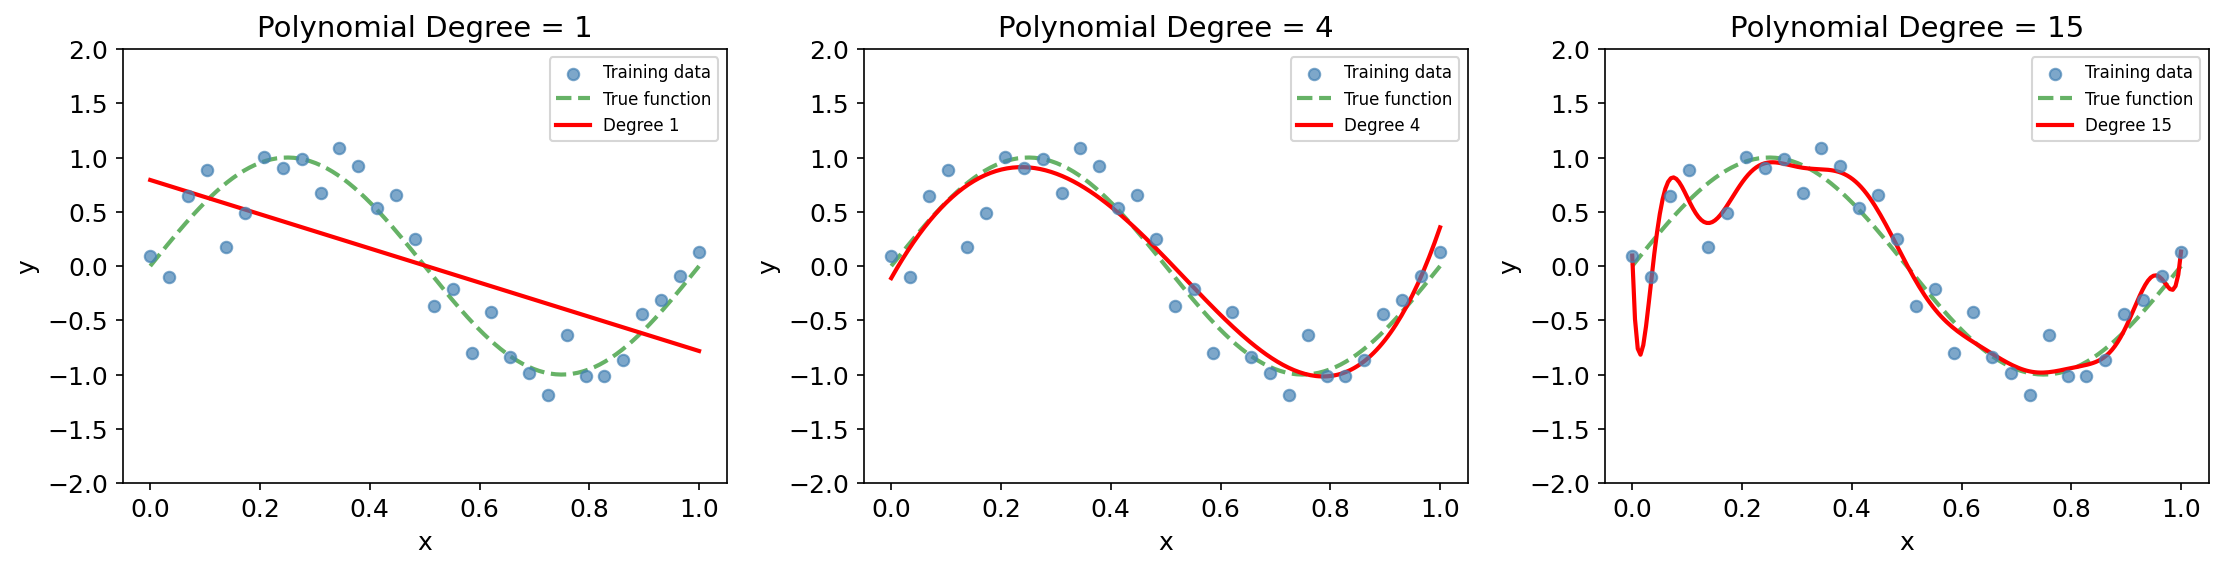
\includegraphics[width=\textwidth]{figures/polynomial_fits.png}
    \caption{Polynomial fits at degree 1 (underfitting), 4 (good fit), and 15 (overfitting).}
    \label{fig:polynomial-fits}
\end{figure}

\subsection{Training vs. Test Error}

Figure~\ref{fig:error-complexity} shows the classic U-shaped test error curve.
Training error (blue) decreases monotonically as degree increases --- a
higher-degree polynomial always fits the training data better. Test error (red),
however, first decreases as the model gains capacity to approximate $\sin(2\pi x)$,
then sharply increases as the model begins fitting noise.

The minimum test error occurs around degree 3--5, confirming that moderate complexity
is optimal. Beyond degree 10, test error grows exponentially due to the numerical
instability of high-degree polynomial coefficients --- a practical hazard of
overfitting.

\begin{figure}[H]
    \centering
    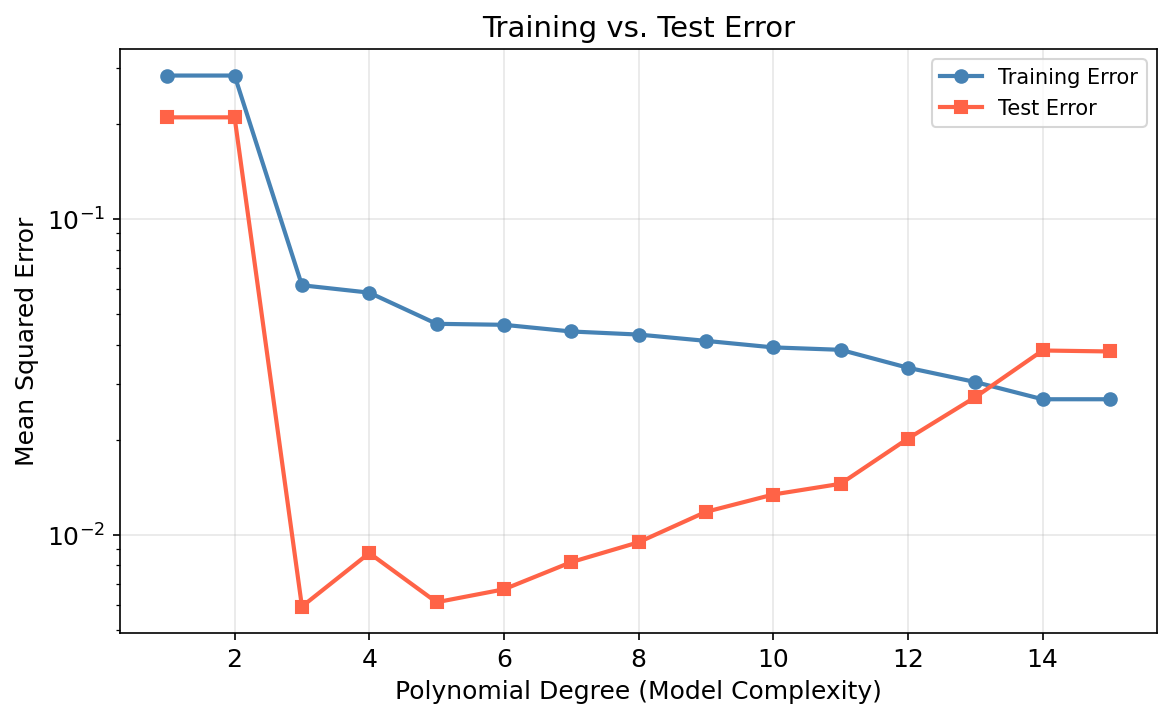
\includegraphics[width=0.8\textwidth]{figures/error_vs_complexity.png}
    \caption{Training and test error as a function of polynomial degree.}
    \label{fig:error-complexity}
\end{figure}

\subsection{Bias-Variance Decomposition: Empirical Verification}

To empirically verify the bias-variance decomposition (Equation~\ref{eq:bias-variance}),
we perform a Monte Carlo simulation: 200 independent datasets are generated, a
polynomial is fitted on each, and the bias$^2$ and variance are estimated from the
spread of predictions at fixed test points.

Figure~\ref{fig:bias-variance} confirms the theoretical prediction. At low degrees
(left side), bias dominates --- the model is too simple. At high degrees (right side),
variance dominates --- the model changes dramatically with each new training sample.
The total error curve shows a clear minimum near degree 3--4, matching the test error
minimum from Section~\ref{sec:experiments}.

\begin{figure}[H]
    \centering
    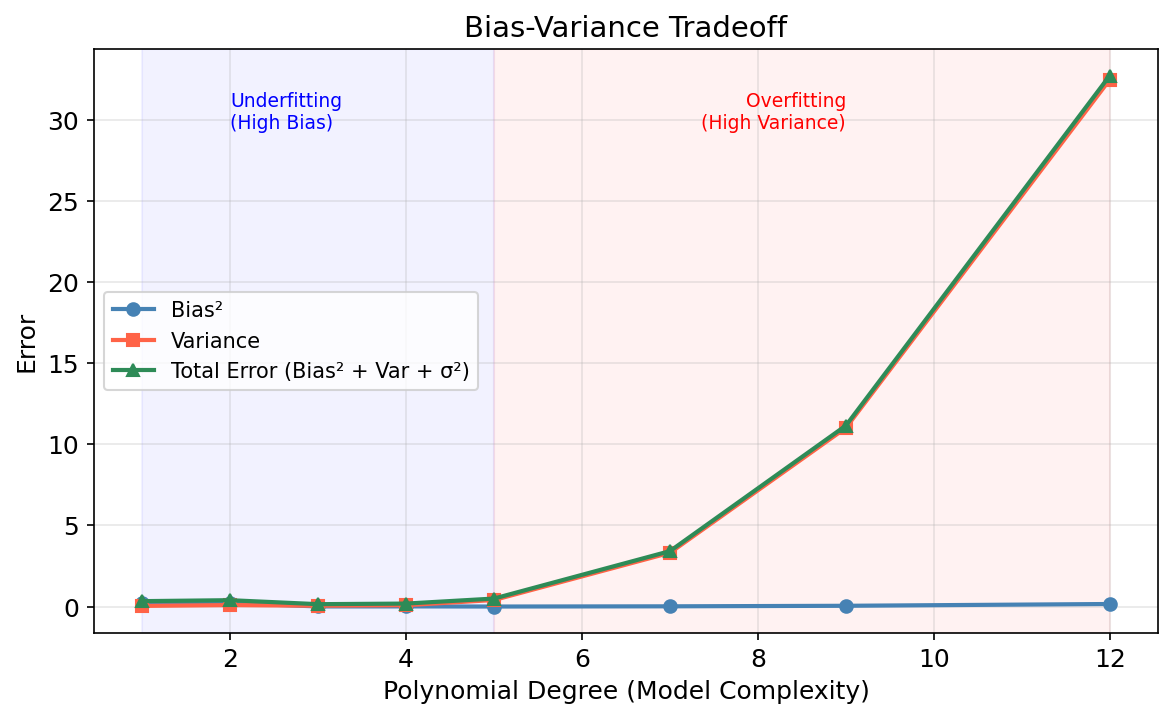
\includegraphics[width=0.8\textwidth]{figures/bias_variance_tradeoff.png}
    \caption{Empirical bias-variance tradeoff estimated via Monte Carlo simulation.}
    \label{fig:bias-variance}
\end{figure}

% ============================================
\section{Solutions: Regularization}
\label{sec:regularization}

\subsection{Ridge Regression (L2 Regularization)}

The Ridge objective adds an L2 penalty:
\begin{equation}
\min_{\mathbf{w}} \| \mathbf{y} - \mathbf{X}\mathbf{w} \|_2^2 + \alpha \|\mathbf{w}\|_2^2
\label{eq:ridge}
\end{equation}

The closed-form solution is:
\begin{equation}
\mathbf{w}_{\text{ridge}} = (\mathbf{X}^\top \mathbf{X} + \alpha \mathbf{I})^{-1} \mathbf{X}^\top \mathbf{y}
\end{equation}

Compared with the ordinary least squares solution $(\mathbf{X}^\top \mathbf{X})^{-1} \mathbf{X}^\top \mathbf{y}$,
the Ridge solution adds $\alpha \mathbf{I}$ to the normal equations, which has two effects:
(1) it ensures the matrix is invertible even when $\mathbf{X}^\top \mathbf{X}$ is
ill-conditioned, and (2) it shrinks all coefficients toward zero by an amount proportional
to $\alpha$ \citep{hoerl1970ridge}.

Geometrically, the Ridge penalty constrains the solution to lie within an $\ell_2$-ball
of radius inversely related to $\alpha$. As $\alpha$ increases, the ball shrinks and
coefficients are more aggressively dampened.

Figure~\ref{fig:ridge} shows this effect on degree-10 polynomial features. At very low
$\alpha$ (left), the model overfits and test error is high. As $\alpha$ increases, test
error first drops (regularization suppresses noise-fitting) then rises (too much
regularization causes underfitting). The right panel confirms that coefficient norms
shrink monotonically with $\alpha$.

\subsection{Lasso Regression (L1 Regularization)}

The Lasso objective adds an L1 penalty:
\begin{equation}
\min_{\mathbf{w}} \| \mathbf{y} - \mathbf{X}\mathbf{w} \|_2^2 + \alpha \|\mathbf{w}\|_1
\label{eq:lasso}
\end{equation}

Unlike Ridge, the $\ell_1$ penalty in Lasso produces \emph{sparse} solutions: many
coefficients are driven exactly to zero \citep{tibshirani1996regression}. This makes
Lasso simultaneously a regularization method and a feature selection technique.

The geometric intuition is that the $\ell_1$-ball has corners aligned with the
coordinate axes. The constrained optimum tends to land on these corners, zeroing out
coefficients corresponding to unimportant features.

Figure~\ref{fig:lasso} shows the Lasso error curve and coefficient shrinkage. The
behavior is qualitatively similar to Ridge, but the coefficient norm drops more
abruptly. Figure~\ref{fig:ridge-vs-lasso} provides a direct comparison at
$\alpha = 0.01$: Ridge shrinks all 10 polynomial coefficients smoothly, while
Lasso sets several of them exactly to zero, retaining only the most informative terms.

\subsection{Experimental Results}

\begin{figure}[H]
    \centering
    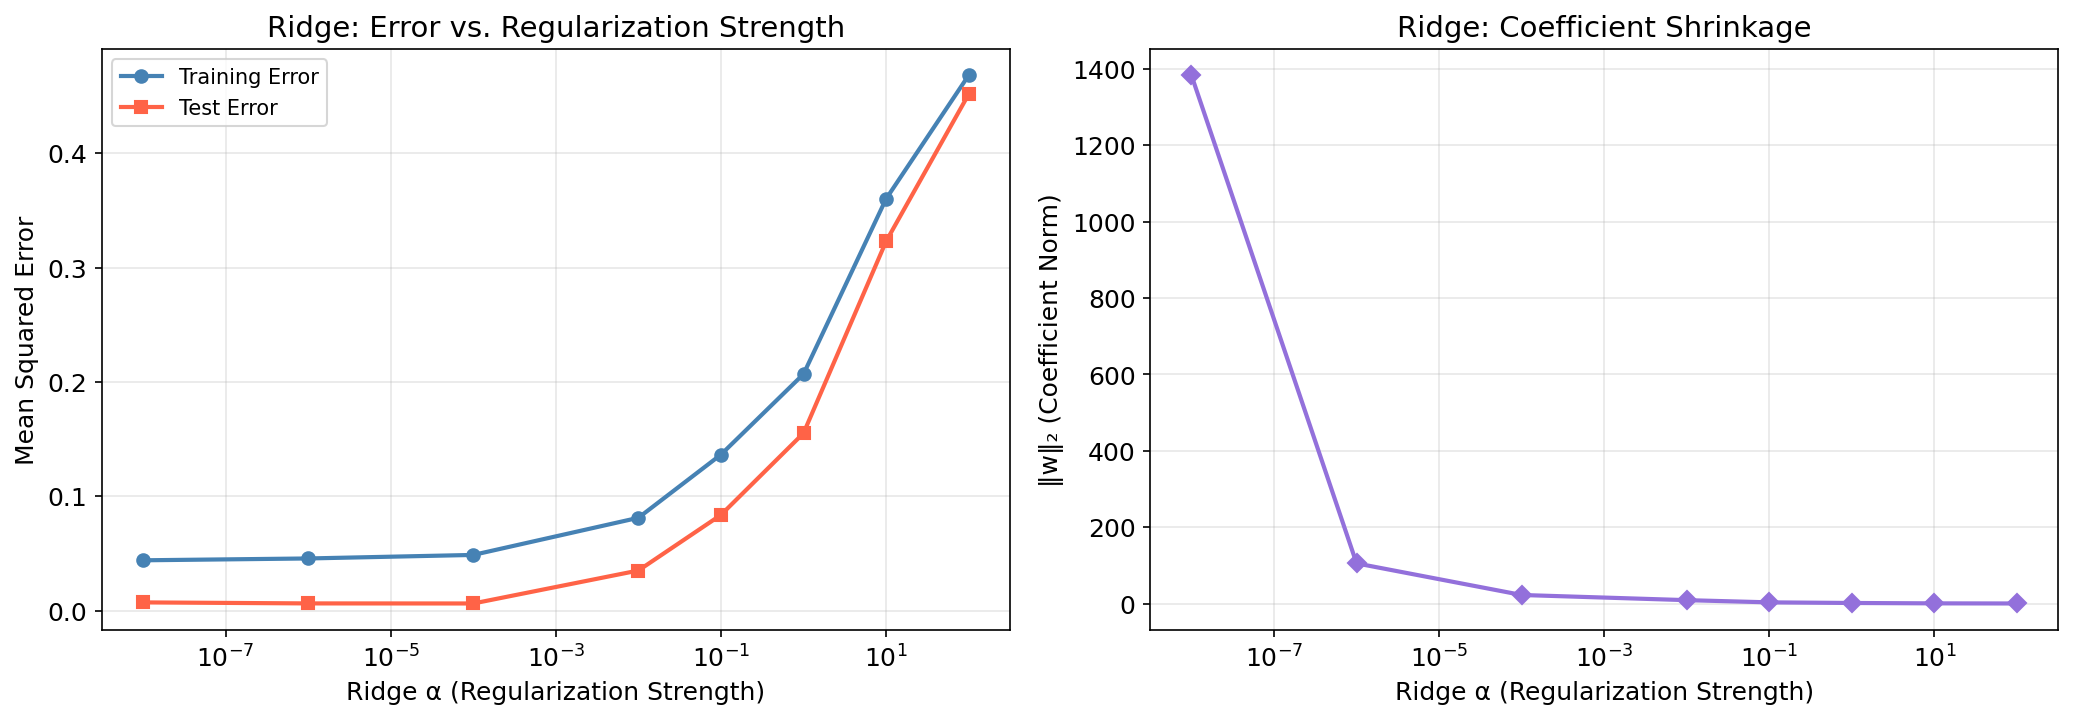
\includegraphics[width=\textwidth]{figures/ridge_regularization.png}
    \caption{Ridge regression: error and coefficient norm vs. regularization strength.}
    \label{fig:ridge}
\end{figure}

\begin{figure}[H]
    \centering
    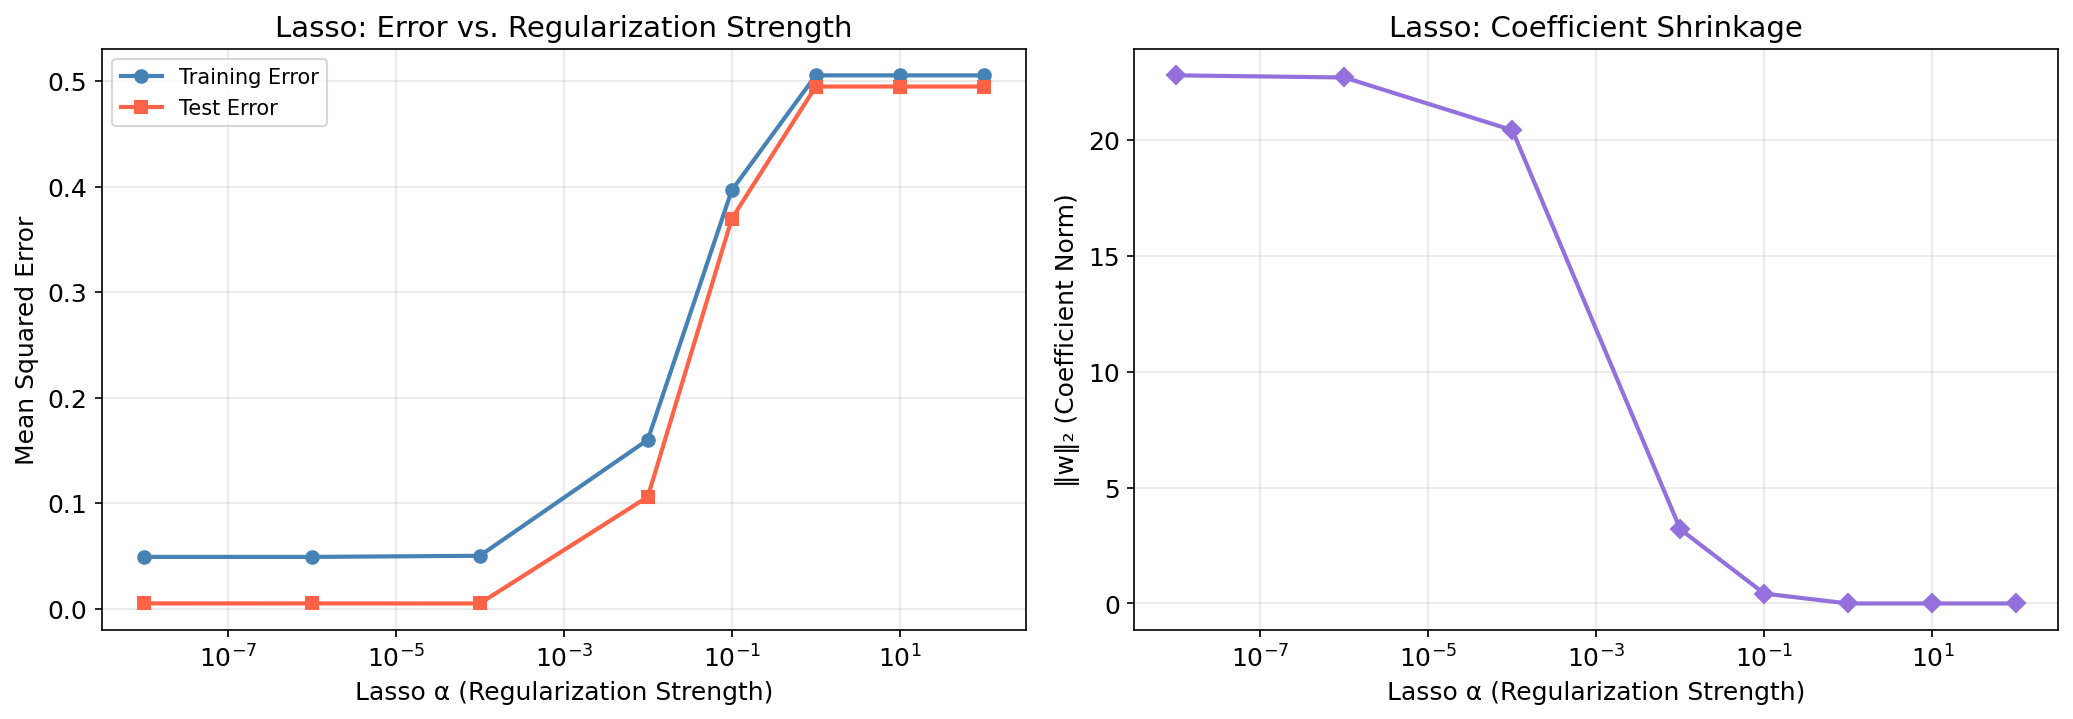
\includegraphics[width=\textwidth]{figures/lasso_regularization.png}
    \caption{Lasso regression: error and coefficient norm vs. regularization strength.}
    \label{fig:lasso}
\end{figure}

\begin{figure}[H]
    \centering
    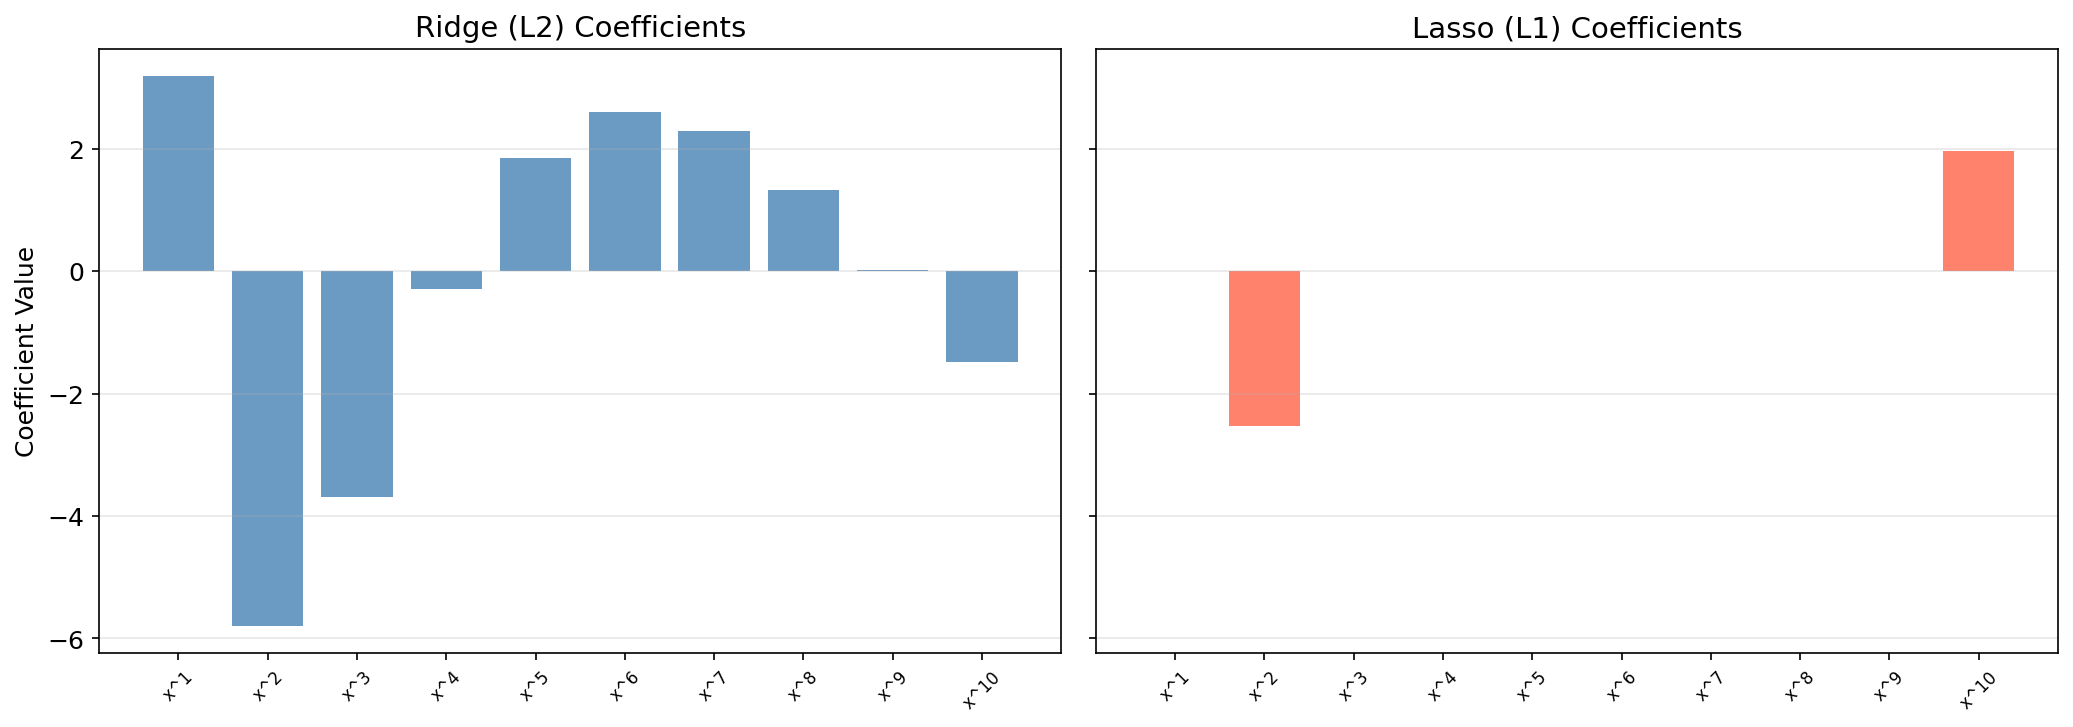
\includegraphics[width=\textwidth]{figures/ridge_vs_lasso_coefficients.png}
    \caption{Ridge vs. Lasso: coefficient comparison at $\alpha = 0.01$.}
    \label{fig:ridge-vs-lasso}
\end{figure}

\subsection{Cross-Validation}

The regularization parameter $\alpha$ controls the bias-variance tradeoff, but its
optimal value depends on the data and cannot be determined analytically.
\emph{$K$-fold cross-validation} is the standard approach for selecting $\alpha$
\citep{hastie2009elements}:

\begin{enumerate}
    \item Partition the training data into $K$ equal-sized folds.
    \item For each fold $k$, train the model on the remaining $K-1$ folds and evaluate
          on fold $k$.
    \item Average the $K$ evaluation scores to obtain a cross-validation estimate of
          test error.
    \item Select the $\alpha$ that minimizes this estimate.
\end{enumerate}

Typical choices are $K = 5$ or $K = 10$. Cross-validation provides an unbiased estimate
of generalization error without requiring a separate validation set, making it
particularly valuable when data is scarce.

\subsection{Other Techniques}

\textbf{Early Stopping.}
During iterative training (e.g., gradient descent on neural networks), training error
decreases monotonically, but test error eventually begins to rise. Early stopping halts
training at the epoch where test error is minimized, effectively limiting model
complexity by restricting the number of optimization steps. This is equivalent to an
implicit form of regularization \citep{goodfellow2016deep}.

\textbf{Dropout.}
Dropout \citep{srivastava2014dropout} randomly sets each hidden unit to zero with
probability $p$ during training, forcing the network to learn redundant representations.
At test time, all units are active but their outputs are scaled by $(1-p)$. This acts as
an ensemble of sub-networks and significantly reduces overfitting, particularly in large
networks trained on limited data.

Both techniques are demonstrated experimentally in Section~\ref{sec:application}.

% ============================================
\section{Application in AI}
\label{sec:application}

Deep neural networks present a paradox: they have far more parameters than training
examples, yet often generalize well. \citet{zhang2021understanding} showed that deep
networks can memorize random labels, demonstrating that their capacity alone does not
explain generalization --- the optimization procedure and implicit regularization play
critical roles.

\subsection{Network Architecture and Overfitting}

Figure~\ref{fig:dl-synthetic} shows MLP regression on the same $\sin(2\pi x)$ data used
in Section~\ref{sec:experiments}. A shallow network (8 hidden units) underfits, while a
deep network (4 hidden layers, 128--16 units) overfits with visible oscillations ---
directly paralleling the polynomial degree experiment.

\begin{figure}[H]
    \centering
    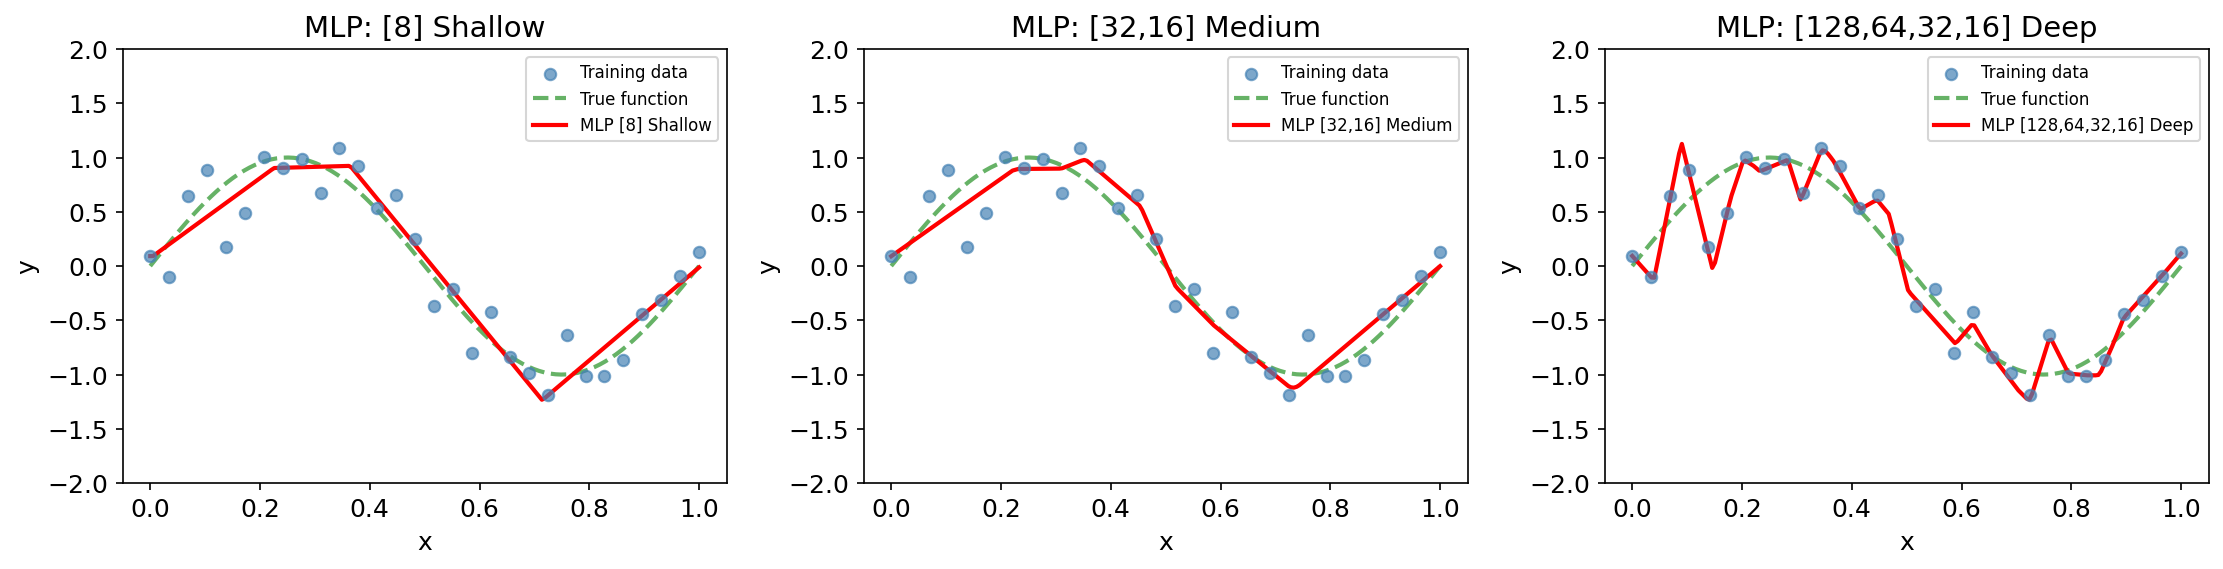
\includegraphics[width=\textwidth]{figures/dl_synthetic_overfitting.png}
    \caption{MLP regression on $\sin(2\pi x)$: shallow (8 units), medium (32-16), and deep (128-64-32-16) architectures.}
    \label{fig:dl-synthetic}
\end{figure}

Figure~\ref{fig:dl-complexity} systematically varies network size. Like polynomial
degree, increasing parameters first improves then degrades test performance, confirming
that the bias-variance tradeoff applies to neural networks.

\begin{figure}[H]
    \centering
    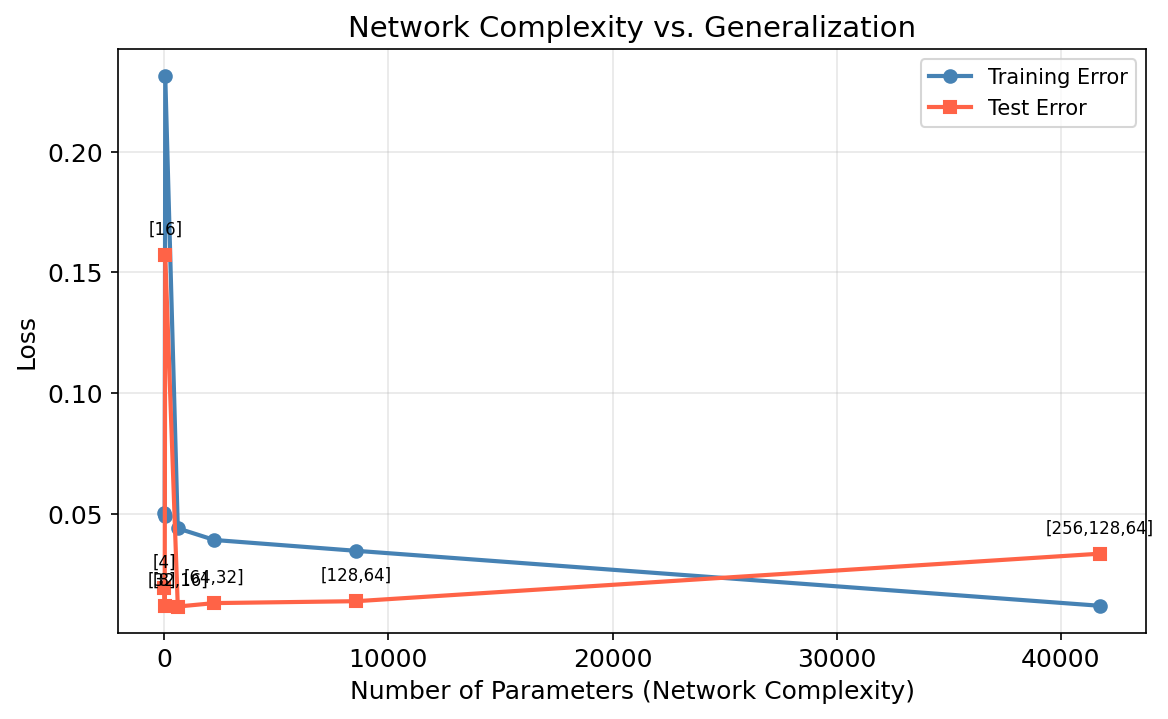
\includegraphics[width=0.8\textwidth]{figures/dl_network_complexity.png}
    \caption{Network complexity (parameter count) vs. train and test error for MLP regression.}
    \label{fig:dl-complexity}
\end{figure}

\subsection{Early Stopping in Practice}

Figure~\ref{fig:dl-curves} shows training and test loss curves for the deep network.
Test loss reaches a minimum early in training (green marker), after which further
training memorizes noise. Early stopping at this point recovers near-optimal
generalization without modifying the architecture.

\begin{figure}[H]
    \centering
    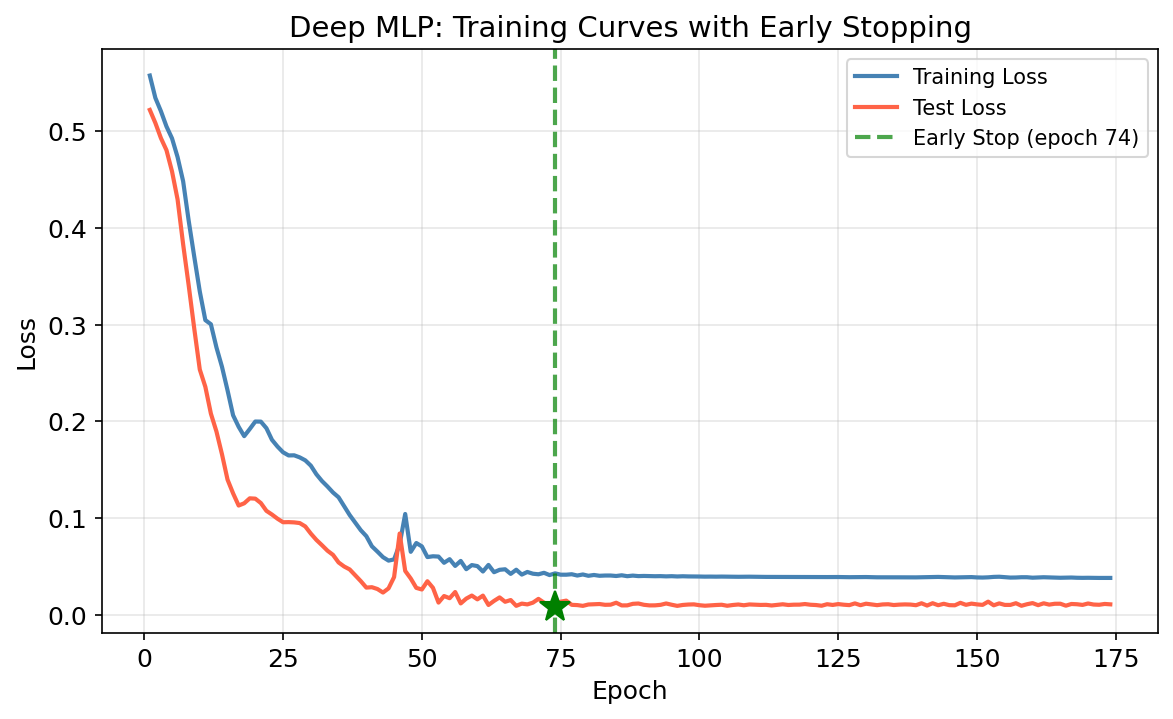
\includegraphics[width=0.8\textwidth]{figures/dl_training_curves.png}
    \caption{Deep MLP training curves. The green marker indicates the early stopping point where test loss is minimized.}
    \label{fig:dl-curves}
\end{figure}

\subsection{Dropout as Neural Network Regularization}

We trained a two-layer MLP (256-128) on 500 MNIST training images --- a deliberately
small dataset to induce overfitting. Figure~\ref{fig:dl-dropout} compares training with
and without dropout ($p = 0.5$):
\begin{itemize}
    \item \textbf{Without dropout:} Training loss drops to near zero while test loss
          stagnates, indicating severe overfitting.
    \item \textbf{With dropout:} The gap between training and test loss is smaller,
          demonstrating improved generalization despite the same network capacity.
\end{itemize}

\begin{figure}[H]
    \centering
    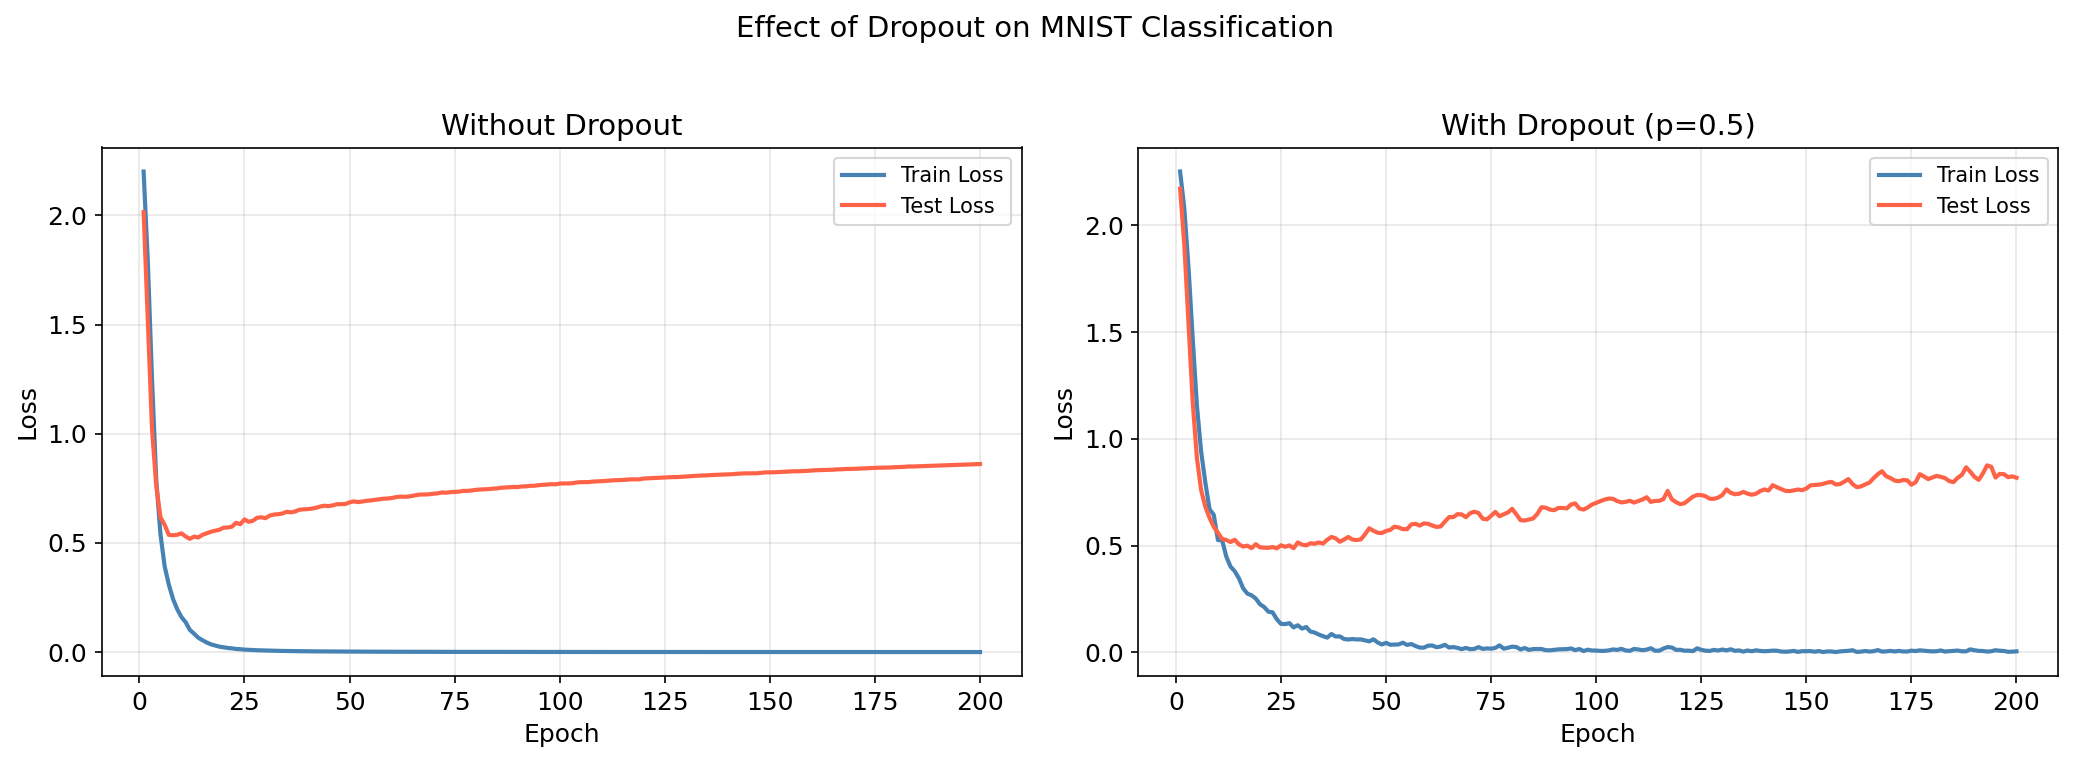
\includegraphics[width=\textwidth]{figures/dl_dropout_effect.png}
    \caption{MNIST classification (500 training samples): overfitting without dropout (left) vs. regularized training with dropout $p=0.5$ (right).}
    \label{fig:dl-dropout}
\end{figure}

\subsection{Other Deep Learning Regularization}

Beyond early stopping and dropout, modern deep learning employs additional techniques:
\begin{itemize}
    \item \textbf{Weight decay} ($\ell_2$ regularization on network weights) mirrors
          Ridge regression.
    \item \textbf{Data augmentation} artificially increases training set size through
          transformations (rotations, crops, flips).
    \item \textbf{Batch normalization} stabilizes training and has an implicit
          regularization effect.
\end{itemize}
These methods are often combined in practice, with the optimal recipe depending on the
specific dataset and architecture \citep{goodfellow2016deep}.

% ============================================
\section{Conclusion}
\label{sec:conclusion}

This report has examined overfitting and underfitting through a unified lens spanning
classical statistics and modern deep learning. Our key findings are:

\begin{enumerate}
    \item The bias-variance decomposition provides the theoretical foundation: underfitting
          corresponds to high bias, overfitting to high variance, and the optimal model
          balances both (Section~\ref{sec:theory}).
    \item Polynomial regression experiments clearly demonstrate the U-shaped test error
          curve and confirm the bias-variance tradeoff empirically via Monte Carlo
          simulation (Section~\ref{sec:experiments}).
    \item Regularization techniques --- Ridge ($\ell_2$) and Lasso ($\ell_1$) --- control
          overfitting by penalizing model complexity, with Lasso additionally performing
          feature selection (Section~\ref{sec:regularization}).
    \item In deep learning, early stopping and dropout serve analogous roles, controlling
          effective model complexity during training (Section~\ref{sec:application}).
\end{enumerate}

\textbf{Practical guidelines:}
\begin{itemize}
    \item Start with a simple model and increase complexity only as needed.
    \item Always evaluate on held-out data; use cross-validation for hyperparameter selection.
    \item Apply regularization (Ridge/Lasso for linear models; dropout/weight decay for
          neural networks) as a default practice.
    \item Monitor training curves: a growing gap between training and test error is the
          earliest sign of overfitting.
\end{itemize}

% ============================================
\bibliographystyle{plainnat}
\bibliography{references}

\end{document}
